\chapter{Basis and modelling}
\section{UAV model}
A fixed wing \gls{uav} model is presented in \citep{beard2012small}, which contain the kinetic equations of a general \gls{mav}. The kinetic equations used to described a general \gls{mav} can represent a fixed wing \gls{uav} given that the size of the \gls{uav} is small enough, which is the case with the \gls{uav} used in this thesis. First the kinematic equations used to describe a \gls{mav} are given as:
\begin{subequations}
\label{eq:kinematics}
\begin{align}\label{eq:kinematicsPosition}
& \begin{bmatrix}
\dot{x} \\
\dot{y} \\
\dot{z}
\end{bmatrix}
=
 \mathbf{R}(\mathbf{\Theta})_{Body}^{NED}\begin{bmatrix}
 u \\
 v \\
 w
 \end{bmatrix} \\
& \begin{bmatrix}
\dot{\phi} \\
\dot{\theta} \\
\dot{\psi}
\end{bmatrix}
= 
\mathbf{T}(\mathbf{\Theta}_{nb})\begin{bmatrix}
p \\
q \\
r
\end{bmatrix}\label{eq:kinematicsAttitude}
\end{align}
\end{subequations}
where $\mathbf{R}(\mathbf{\Theta})_{Body}^{NED}$ is the rotation matrix from the body frame to the NED frame, with $\mathbf{\Theta} = \begin{bmatrix}
\phi & \theta & \psi
\end{bmatrix}^T.$ The transformation matrix $\mathbf{T}(\mathbf{\Theta}_{nb})$ is given in \citep{fossen2011handbook} as:
\begin{equation}
\mathbf{T}(\mathbf{\Theta}_{nb}) = \begin{bmatrix}
1 & \sin(\phi)\tan(\theta) & \cos(\phi)\tan(\theta) \\
0 & \cos(\phi) & -\sin(\phi) \\
0 & \frac{\sin(\phi)}{\cos(\theta)} & \frac{\cos(\phi)}{\cos(\theta)}
\end{bmatrix}
\end{equation}
The kinetic equations presented from \citep{beard2012small} is given in the body frame, which is a frame fixed to the body of the vehicle and rotated relative to an inertia frame, e.q the Earth center. The kinetic equations are given as:
\begin{subequations}
\label{eq:kinetics}
\begin{align}
\begin{bmatrix}
F_x \\
F_y \\
F_z
\end{bmatrix}
&= \mathbf{R}(\mathbf{\Theta})^{Body}_{NED}\begin{bmatrix}
0 \\
0 \\
mg
\end{bmatrix} - \frac{1}{2} \rho V_a^2 S \mathbf{R}(\alpha)_{Stability}^{Body}\begin{bmatrix}
F_{Drag} \\
0 \\
F_{Lift}
\end{bmatrix}\\ &+ \frac{1}{2} \rho V_a^2 S \begin{bmatrix}
0 \\
C_y(\beta,p,r,\delta_a,\delta_r) \notag\\
0
\end{bmatrix} + \frac{1}{2} \rho S_{Prop} C_{Prop} \begin{bmatrix}
(K_{Motor}\delta_t)^2-V_a^2 \\
0 \\
0
\end{bmatrix}\\
\begin{bmatrix}
 L \\
 M \\
 N 
 \end{bmatrix} &= \frac{1}{2} \rho V_a^2S\begin{bmatrix}
 C_L(\beta,p,r,\delta_a,\delta_r) \\
 C_M(\alpha,q,\delta_e) \\
 C_N(\beta,p,r,\delta_a,\delta_r)
 \end{bmatrix} + \begin{bmatrix}
 -k_{T_p}(K_\Omega\delta_t)^2 \\
 0 \\
 0
 \end{bmatrix}
\end{align}
\end{subequations}
where $\rho$ is the air density in $kg/m^3$,$mg$ is the weight of the \gls{mav}, $S$ is the platform area of the \gls{mav} wing, $C_i$ are nondimensional aerodynamic coefficients and $V_a$ is the speed of the \gls{mav} through the surrounding air. $\alpha$ and $\beta$ is the attack and side slip angle respectfully. $F_{Drag}$ is the drag force acting on the fuselage, and $F_{Lift}$ is the lift force. $\mathbf{R}(\alpha)_{Stability}^{Body}$ are the rotation matrix from the stability frame to the body frame. The stability frame is orientated with respect to the \gls{mav} movement through the surrounding air, which is defined as a standard rotation around the y-axis of the body frame. $S_{Prop}$ is the area swept out by the propeller, and $K_{Motor}$,$K_{T_p}$ and $K_\Omega$ are propeller specific constants. The control surface on the \gls{mav} is defined into two groups; the wings and the rudder. On the rudder $\delta_e$ controls the elevator deflection and $\delta_r$ the rudder deflection. For the wings $\delta_a$ is the control input from the aileron deflection, while $\delta_t$ is the throttle control input.
\section{Landing path modelling}
A landing path can be view as a path following problem, which is the \gls{uav} attempts to follow a desired path without a time demand. A minimum requirement for a path is that the path is connected, where the connection level can be described by the path smoothness. Smoothness can be described with parametric continuity, which is denoted $C^n$ were n is the degree of smoothness. The order of n implies that the n first parametric derivatives match at a common point for two subsequent paths \citep{barsky1989geometric}. Geometric continuity is a relaxed form of parametric continuity in which discontinuousness in speed is allowed. A table \ref{TB:SmoothnessDescriptions} of geometric and parametric continuity lists the requirement for each smoothness level, which is based definitions presented in \citep{barsky1989geometric}. Geometric continuity is sufficient for a path following system, which is the main focus of this thesis. Geometric continuity is denoted as $G^n$ were n is the order of continuity.
\begin{table}[H]
\begin{center}
\begin{tabular}{| l | l |}
\hline
\textbf{Geometrical smoothness level} & \textbf{Description} \\ \hline
$G^0$ & All subpaths are connected \\ \hline
$G^1$ & The path-tangential angle is continuous \\ \hline
$G^2$ & The center of curvature is continuous \\ \hline
\textbf{Parametric smoothness level} & \textbf{Description} \\ \hline
$C^0$ & All subpaths are connected \\ \hline
$C^1$ & The velocity is continuous \\ \hline
$C^2$ & The acceleration is continuous \\ \hline
\end{tabular}
\end{center}
\caption{Smoothness definitions for both parametric and geometric}
\label{TB:SmoothnessDescriptions}
\end{table} 
The definition used for path in this thesis is equation 1.2 in \citep{tsourdos2010cooperative} which state:
\begin{equation}
P_s(x_s,y_s,z_s,\theta_s,\psi_s) \xrightarrow{r(\varpi)} P_f(x_f,y_f,z_f,\theta_f,\psi_f)
\end{equation}
where the subscripts $s$ and $f$ denotes the start pose and finish pose respectfully with $r(\varpi)$ as the path and $\varpi$ the path variable.

\subsection{Straight lines}
The simplest path from $P_s$ and $P_f$ is a straight line path between the poses. A straight line path is given, where for for simplicity and without loss of generality the path is reduced to a 2 dimensional case: 
\begin{subequations}
\begin{align}
& x(\varpi) = a_x\varpi + b_x \\
& y(\varpi) = a_y\varpi + b_y 
\end{align}
\end{subequations}
with $ \varpi \in [0,1] $, where $\varpi$ has not necessary a physical meaning. Then the parametrisation of the straight line becomes:
\begin{subequations}
\begin{align}
P(0) &= \begin{bmatrix}
x(0) \\
y(0)
\end{bmatrix} = \begin{bmatrix}
b_x \\
b_y
\end{bmatrix} = \begin{bmatrix}
x_s \\
y_s
\end{bmatrix} \\
P(1) &= \begin{bmatrix}
x(1) \\
y(1)
\end{bmatrix} = \begin{bmatrix}
a_x + b_x \\
a_y + b_y
\end{bmatrix} = \begin{bmatrix}
x_f \\
y_f
\end{bmatrix} \rightarrow \begin{bmatrix}
a_x \\
a_y
\end{bmatrix} = \begin{bmatrix}
x_f - b_x \\
y_f - b_y
\end{bmatrix}
\end{align}
\end{subequations}
Further the path tangential for a straight line path is given as:
\begin{equation}
\psi(\varpi) = \atan2(a_y,a_x)
\end{equation}
which shows that the path-tangential for a straight line path is discontinues, as seen in figure \ref{Fig:Path-tangential}. That define a straight line path with the smoothness of $G^0$, which allows the path to be used in a path following system, however with discontinuity in the path-tangential. A straight line path is shown in  figure \ref{Fig:StraightLinePath}.
\begin{figure}[H]
\centering
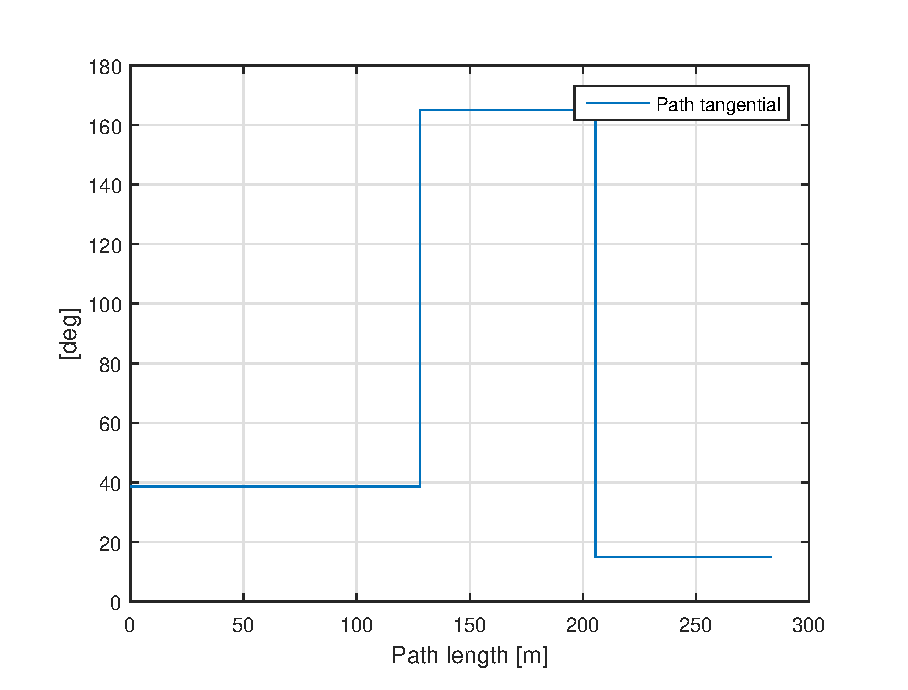
\includegraphics[scale=0.5]{figs/TheoryPlot/TangentialStraight.eps}
\caption{Path-tangential to a straight line path}
\label{Fig:Path-tangential}
\end{figure}
\begin{figure}[H]
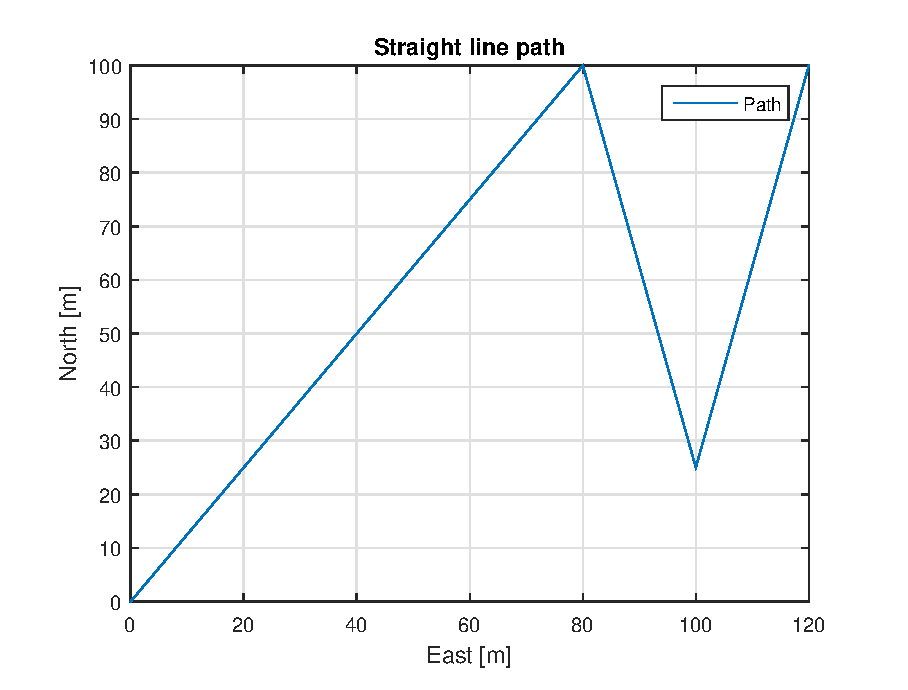
\includegraphics[width=0.5\textwidth]{figs/TheoryPlot/StraightLine.eps}
\caption{Straight line path}
\label{Fig:StraightLinePath}
\end{figure}
\subsection{Dubins path}\label{S:DubinsPath}
An alternative to a straight line path is a path constructed by straight lines and circle, like the Dubins path proposed in the paper \citep{dubins1957curves}, which showed that the shortest possible path for a particle that moved with unit speed with maximum curvature would consist of two circles and a straight line which is tangential to both circles.


 

A Dubins path which is constructed with the final orientation fixed has four ways to be constructed, which are determined by the rotation directions. The four rotation combination with fixed finish orientation are given in table \ref{Tb:DubinsTurningDirection}.
\begin{table}[H]
\centering
\begin{adjustbox}{max width=\textwidth}
\begin{tabular}{ | l |}
\hline
Right to Right \\
Right to left \\
Left to Right \\
Left to left \\ \hline
\end{tabular}
\end{adjustbox}
\caption{Turning direction for Dubins path with fixed final orientation}
\label{Tb:DubinsTurningDirection}
\end{table}
The equations used to construct a Dubins path are found in \citep{tsourdos2010cooperative} section 2.2.1, with a constructed path shown in figure \ref{Fig:DubinsPath}. In figure \ref{Fig:DubinsPath} the whole line is the path, with the doted lines used express the parameter used to construct the path.
\begin{figure}[H]
\def\svgwidth{\textwidth} % Defining the width since Inkscape hasn't done this yet in the .pdf_tex file
\input{InkFig/DubinsPath.pdf_tex}
\caption{The whole line is the Dubins path, while the doted lines are used to express the parameter used to construct the path}
\label{Fig:DubinsPath}
\end{figure}
Dubins path is constructed by first determine the start and finish turning circle center. The centres are found with the equations:
\begin{subequations}
\begin{align}
X_{cs} &= X_s - R_s\cos(\psi_s \pm \frac{\pi}{2}) \\
Y_{cs} &= Y_s - R_s\sin(\psi_s \pm \frac{\pi}{2}) \\
X_{cf} &= X_f - R_f\cos(\psi_f \pm \frac{\pi}{2}) \\
Y_{cf} &= Y_f - R_f\sin(\psi_f \pm \frac{\pi}{2})
\end{align}
\end{subequations}
where $R_s$ and $R_f$ is the radius of the start and final turning circle respectfully, with $\psi_s$ and $\psi_f$ the start and finish orientation. The centres for the start and finish turning circle are defined as:

\begin{align}
& \mathbf{O}_{cs} =
\begin{bmatrix}
X_{cs} \\
Y_{cs}
\end{bmatrix} \\
& \mathbf{O}_{cf} =
\begin{bmatrix}
X_{cf} \\
Y_{cf}
\end{bmatrix}
\end{align}
Continuing the centres $O_{cs}$ and $O_{cf}$ are connected with a centreline $c$, where the length is given as:
\begin{equation}
|c| = ||\mathbf{O}_{cs} - \mathbf{O}_{cf}||_2
\end{equation}
where $||\cdot||_2$ is the second norm. Continuing the arc exit and entry point for the start and finish circles are calculated by first applying the equations:
\begin{subequations}
\begin{align}
& \alpha = \arcsin\left(\frac{R_f-R_s}{|c|}\right) \\
& \beta = \arctan\left(\frac{Y_{cf}-Y_{cs}}{X_{cf}-X_{cs}}\right)
\end{align}
\end{subequations}
where $\alpha$ is the angle between the length of the center line between the two circles, and the length of the line from the start circle to the exit tangent point. $\beta$ is the angle of the center line with respect to the inertial frame. The exit and entry tangent point is found with the use of table \ref{Tb:ExitEntryTangent}.
\begin{table}[H]
\begin{center}
\begin{tabular}{ | l | l |}
\hline
& \textbf{Turn angle} \\ \hline
$\phi_{right}$ & $\alpha + \beta + \frac{\pi}{2}$ \\
$\phi_{left}$ & $\beta - \alpha + \frac{3\pi}{2}$ \\ \hline
\end{tabular}
\caption{Turn angle}
\label{Tb:ExitEntryTangent}
\end{center}

\end{table}
With the angle of the exit and entry tangent point the points are given as:
\begin{subequations}
\begin{align}
& x_{P_\chi} = x_{cs} + R_s\cos(\phi) \\
& y_{P_\chi} = x_{cs} + R_s\sin(\phi) \\
& x_{P_N} = x_{cf} + R_f\cos(\phi) \\
& y_{P_N} = x_{cf} + R_f\sin(\phi)
\end{align}
\end{subequations}
which is used to define the exit and entry points as:
\begin{subequations}
\begin{align}
\mathbf{P}_{\chi} &= \begin{bmatrix}
x_{P_\chi} \\
y_{P_\chi}
\end{bmatrix} \\
\mathbf{P}_N &= \begin{bmatrix}
x_{P_N} \\
y_{P_N}
\end{bmatrix}
\end{align}
\end{subequations}
The length of the Dubins path is calculated in three parts. The first the is the arc length from the start pose to the exit tangent point, then the length of the straight line before the arc length from the entry point to the finish pose. The length of the path is given as: 
\begin{equation}
d = R_s\phi_s + d_t + R_f\phi_f
\end{equation}
where $d_t = ||\mathbf{P}_N-\mathbf{P}_{\chi}||_2$, $\phi_s$ and $\phi_f$ is the arc angle for the start and finish circle respectfully. The path-tangential of the Dubins path is given as:
\begin{equation}
\psi = \atan2(1,-tan(\phi))
\end{equation}
which determine that the path-tangential is continues, which makes Dubins path $G^1$. The path-tangential for Dubins path is shown in figure \ref{Fig:Path-tangentialDubin}.
\begin{figure}
\centering
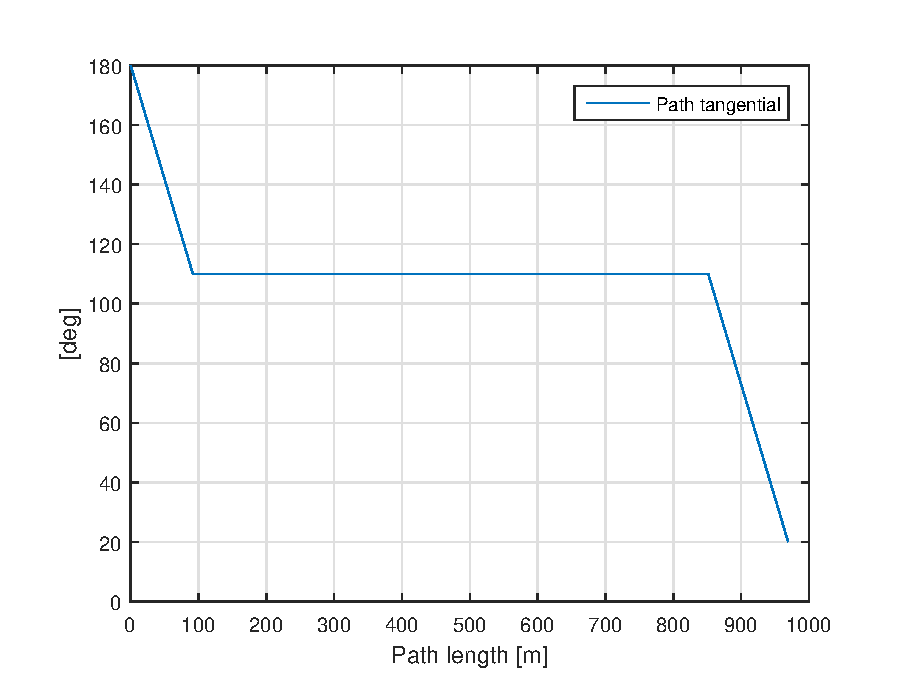
\includegraphics[scale=0.5]{figs/TheoryPlot/tangentialDubin.eps}
\caption{Path-tangential for a Dubins path}
\label{Fig:Path-tangentialDubin}
\end{figure}
\cleardoublepage